\documentclass{beamer}

\usepackage[T1]{fontenc} 
\usepackage[latin1]{inputenc}
%% \usepackage[frenchb]{babel}

\usetheme{Warsaw}

% Supprimer les icones de navigation (pour les transparents)
\setbeamertemplate{navigation symbols}{}

\title[Presentation BioSilico 15 minutes]{Presentation BioSilico 15 minutes}
\author{Gabriel Chandesris}
%% \institute{ --- }
% \institute{ 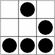
\includegraphics[height=0.5cm]{../img/logo_glider.png} }
\institute{ 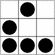
\includegraphics[height=0.5cm]{../img/logo-glider-left.png} 
\includegraphics[height=1.5cm]{../img/digitalBioInfo.jpeg} 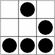
\includegraphics[height=0.5cm]{../img/logo-glider-right.png} }
% \logo{ 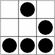
\includegraphics[height=0.5cm]{../img/logo_glider.png} }
\date{ Version : \today } %% \date{\today}

\begin{document}

\begin{frame}
	\titlepage
\end{frame}

\begin{frame}
	\frametitle{Table Of Content}
	\small \tableofcontents[hideallsubsections]
\end{frame} 

\def\titleSectionFirstPart{Starting Ideas}
\section{\titleSectionFirstPart }
\def\titleSubSectionFirstPartOne{ Passion for two domains }
\subsection{ \titleSubSectionFirstPartOne }
\begin{frame}
	\frametitle{ \titleSubSectionFirstPartOne }
	\begin{columns}[T]
	\begin{column}[T]{6.0cm}
		\begin{block}{Computer Software}
			\begin{itemize}
				\item Video Games and "how it works"
				\item Reverse Ingeneering (resources)
				\item Software Development
				\item Programmation
				\item Hack and virus (some readings)
			\end{itemize}
		\end{block}
	\end{column}
	\begin{column}[T]{5.0cm}
		\begin{block}{Biology / Life Sciences }
			\begin{itemize}
				\item Studying Plants and some animals
				\item Biochemistry, genomics, proteomics... 
				\item Modelization and computerization
				\item Uses in Virtual Worlds 
				%% procedural generation && genetic / evolutionary / memetic algorithms
			\end{itemize}
		\end{block}
	\end{column}
	\end{columns}~\\
	\begin{itemize}
		\item SimCity, SimEarth, SimLife... then \emph{Creatures} (1995) !
	\end{itemize}
\end{frame}

\def\titleSectionSecondPart{Next Steps}
\section{\titleSectionSecondPart }
\def\titleSubSectionSecondPartOne{ Gathering information }
\subsection{ \titleSubSectionFirstPartOne }
\begin{frame}
	\frametitle{ \titleSubSectionFirstPartOne }
	\begin{itemize}
		\item Articles, computer software...
		\item ... 
	\end{itemize}
\end{frame}

%% TODO short presentation !!

\def\sectionPartBibliographie{Bibliography / Mediagraphy}
\section{\sectionPartBibliographie}
\begin{frame}
	\frametitle{\sectionPartBibliographie}
	\nocite{*}
	\bibliography{presentationBioSilico15minutes}
	% \bibliographystyle{frplain} % plain or frplain
	\bibliographystyle{plain}
\end{frame}

\end{document}
